\chapter{Monte Carlo Models of Signal and Background} \label{ch:monte_carlo}

\section{Signal Modeling}\label{sec:signal_modeling}

Simulated gluino pair-production events were generated for use in the analysis.
Separate samples were generated for the direct decay and cascade decay models described in~\ref{subsec:rpv_gluino}.
For the direct decay model, events were generated for gluino mass ranging from 900~GeV to 1.8~TeV .
For the cascade model, the gluino mass was varied from 750~GeV up to 2.1~TeV, with the neutralino mass ranging from
450~GeV to 1.9~TeV .
For all signal points, $m_{\tilde{g}} > m_{\tilde{\chi}_1^0}$.
Signal events were simulated for a discrete set of mass points.
Figure~\ref{fig:signal_cascade_grid} indicates the $\left(m_{\tilde{g}}, m_{\tilde{\chi}_1^0}\right)$ points for which
signal evens were generated.

\begin{figure}[!ht]
    \centering
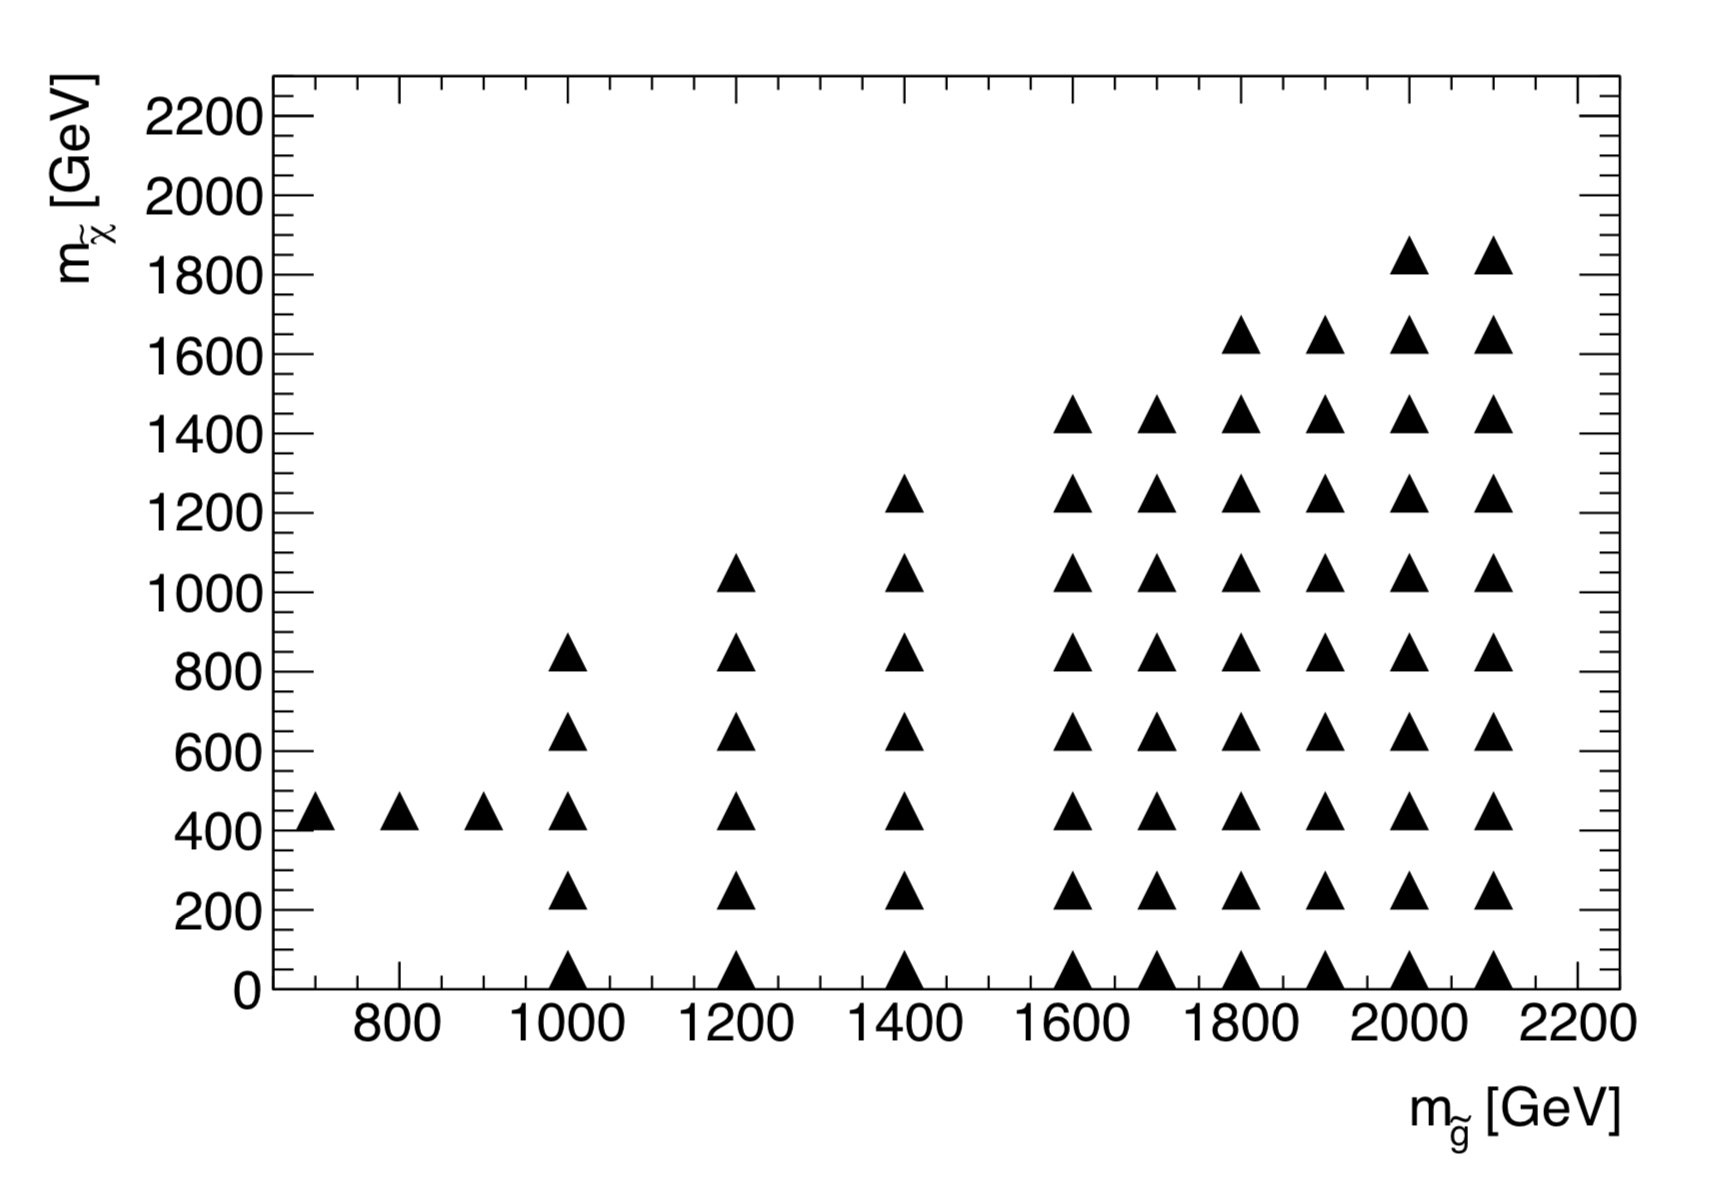
\includegraphics[width=0.8\linewidth]{signal_cascade_grid}
\caption{The grid of gluino and neutralino masses for which simulated cascade decay events were generated. The triangles
indicate the mass points that were generated.}
\label{fig:signal_cascade_grid}
\end{figure}

\subsection{Event generation}\label{subsec:signal_event_gen}

Matrix elements for gluino pair production were generated with \textsc{MadGraph\_aMC@NLO} v2.3.3,
which is a convenient framework for calculating arbitrary matrix elements at up to next-to-leading order (NLO)~\cite{signal-madgraph}.
\textsc{MadGraph} allows the user to specify the theory being used and the values for the free parameters,
and then it constructs and calculates the necessary Feynman diagram.
In this analysis, matrix elements were calculated at leading order (LO).
In the pair-production matrix elements, up two two additional partons were allowed to be produced along with the
gluino pair.

To model the parts of the collision environment described in~\ref{sec:jet_collisions}, such as the underlying event,
parton shower, and fragmentation, \textsc{Pythia} 8.186 is used~\cite{signal-pythia}.

Interfacing \textsc{MadGraph} and \textsc{Pythia} is made possible by a standardized file format known as Les Houches
Event Format (LHEF)~\cite{signal-lhef}.

As discussed in~\ref{sec:jet_collisions}, there are non-perturbative processes that occur in proton-proton collisions,
which cannot be directly calculated from first principles.
This processes can be parameterized and approximated in a program like \textsc{Pythia},
requiring the creation of several free parameters whose values have to be inferred from data.
The process of inferring these parameters so that the calculations match the data is known as tuning.
For this analysis the A14 set of tuned parameter values were used for modeling the underlying event in
\textsc{Pythia}~\cite{signal-pythia-a14,signal-pythia-tunes}.

The parton distribution functions (PDFs) used for the simulated signal generation are from the NNPDF2.3LO
set~\cite{signal-nnpdf}.

\subsection{Cross-section}\label{subsec:signal_cross_section}
In order to estimate the expected signal yield and uncertainty, the nominal production cross section and its uncertainty
must be known.
Gluino pair-production cross-sections have been calculated at a range of center-of-mass energies, and the results
are summarized in~\cite{signal-xsec}.
The gluino pair-production cross-section and its uncertainty over a range of gluino masses can be seen in~\ref{fig:signal_xsec}.

\begin{figure}[!ht]
    \centering
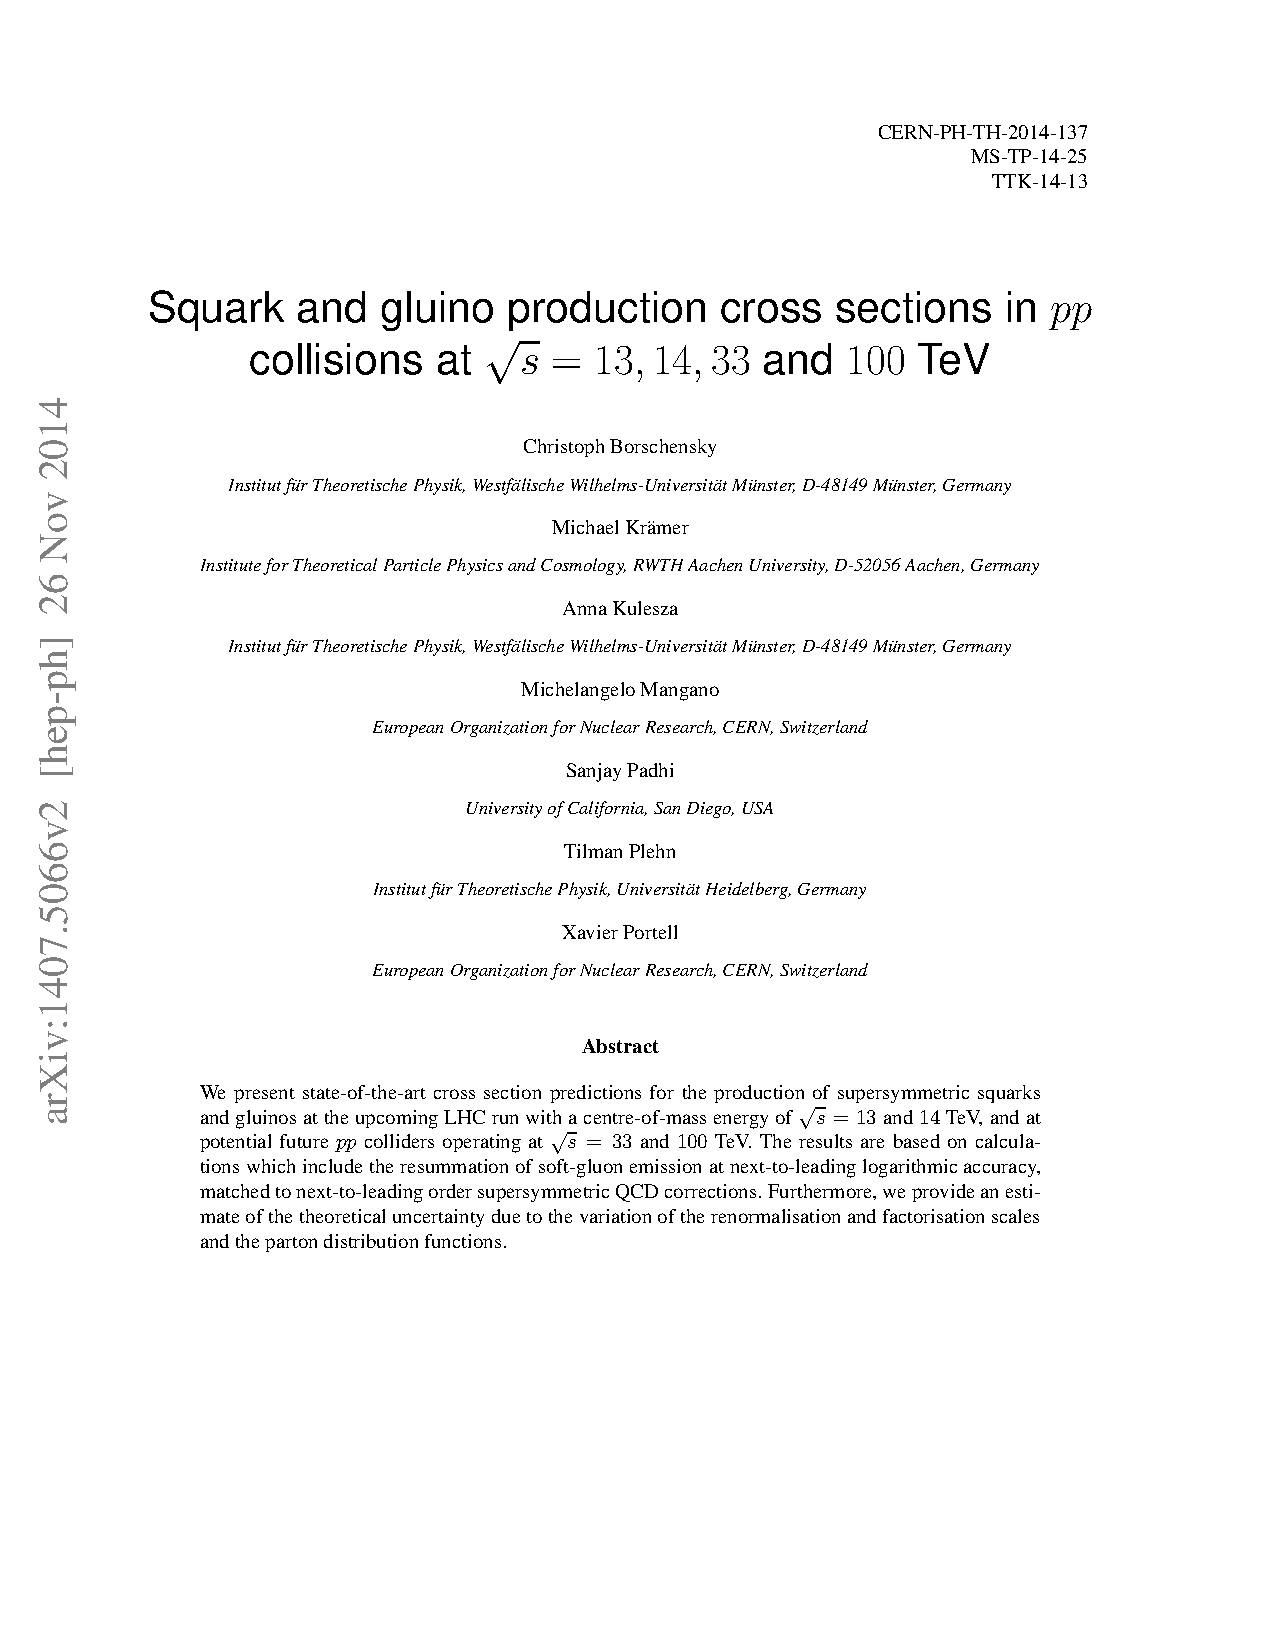
\includegraphics[width=0.8\linewidth]{signal_xsec}
\caption{Gluino pair-production cross-section and uncertainty for $\sqrt{13}~TeV$ proton-proton collisions at the LHC,
calculated at NLO+NLL~\cite{signal-xsec}.}
\label{fig:signal_xsec}
\end{figure}
